\documentclass[tikz, border=10pt]{standalone}
\usepackage{pgfplots}
\usepackage{amsmath}
\usetikzlibrary{backgrounds}
\pgfplotsset{compat=1.18}

\begin{document}
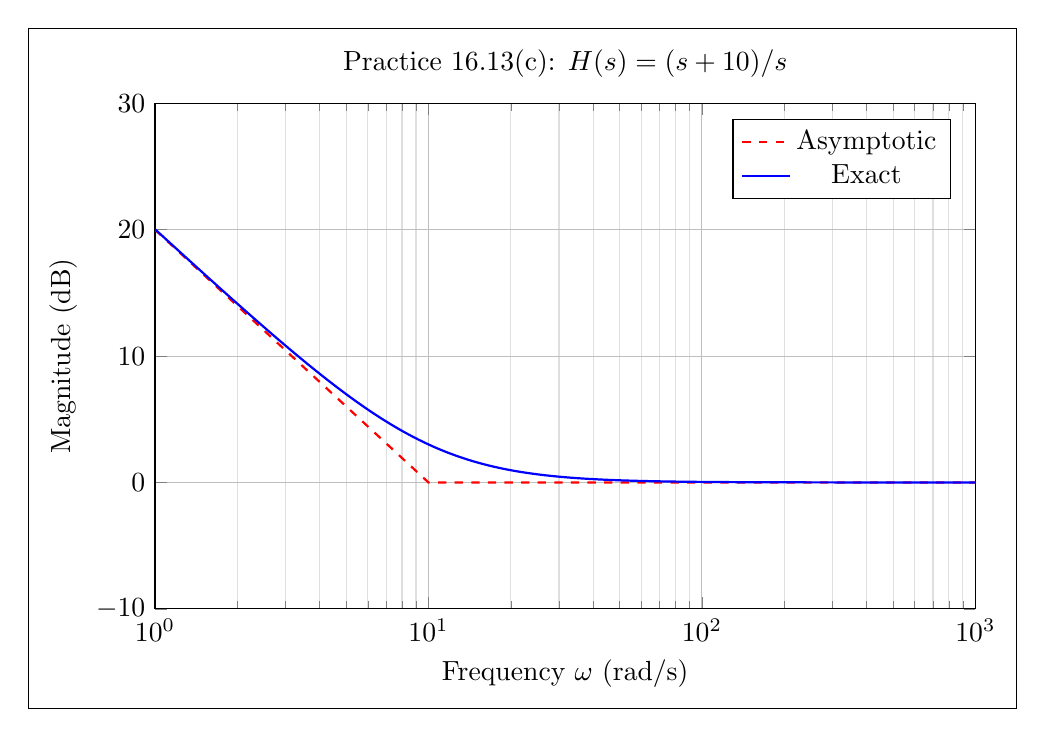
\begin{tikzpicture}[show background rectangle]
    \begin{semilogxaxis}[
        width=12cm, height=8cm,
        title={Practice 16.13(c): $H(s) = (s + 10)/s$},
        xlabel={Frequency $\omega$ (rad/s)},
        ylabel={Magnitude (dB)},
        grid=both,
        xmin=1, xmax=1000,
        ymin=-10, ymax=30,
        minor grid style={gray!25},
        major grid style={gray!50},
        legend pos=north east,
    ]

    % H(s) = (s+10)/s = 10(1 + s/10) / s
    % Zero at 10. Term 10/s => -20 dB/dec passing through 20dB at 1.
    
    % Asymptote
    \addplot[red, dashed, thick] coordinates {
        (1, 20) (10, 0) (1000, 0) 
    };
    \addlegendentry{Asymptotic}

    % Exact
    % 20*log10( sqrt(10^2 + x^2) / x )
    \addplot[blue, thick, domain=1:1000, samples=200] {20*log10(sqrt(100 + x^2)/x)};
    \addlegendentry{Exact}
    
    \end{semilogxaxis}
\end{tikzpicture}
\end{document}
